\chapter{Il progetto di stage}
\label{cap:ilprogettodistage}

In questo capitolo descrivo il progetto di \textit{stage}, e le motivazioni che mi hanno spinto a scegliere questo progetto.\\
Ho scelto {\azienda} perchè è l'azienda per cui lavoro da più di 5 anni, e che mi ha dato la possibilità di crescere professionalmente.
Ho scelto questo progetto perchè mi ha permesso di lavorare con tecnologie nuove, e di imparare nuovi linguaggi di programmazione.\\
Lo \textit{stage} prevedeva lo sviluppo di un prototipo per il monitoraggio, la raccolta e l'analisi delle dipendenze \textit{software} degli applicativi di {\azienda}.\\
Il nome del progetto è \textit{Dependency Analyzer} ed è stato scelto dai membri del team di cui ho fatto parte.\\
\section{Lo \textit{stage} per \azienda}

Gli \textit{stage} rappresentano un pilastro fondamentale nella strategia di {\azienda}, svolgendo molteplici funzioni cruciali. 
Primo fra tutti, offrono l'opportunità di dedicarsi a progetti innovativi che, a causa di limitazioni di \textit{budget} o di tempo, 
non troverebbero spazio nelle attività lavorative ordinarie. I \textit{team} di sviluppo di {\azienda} sono primariamente impegnati 
nel mantenimento e nello sviluppo dei prodotti esistenti, lasciando poco margine per la ricerca e lo sviluppo di nuove idee. 
Questo compito solitamente è affidato al \textit{team} di ricerca e sviluppo, che, nonostante la sua competenza, è spesso limitato dalla scarsità 
di risorse umane per affrontare tutte le richieste innovative. In questo contesto, lo \textit{stage} diventa una soluzione efficace, 
consentendo lo sviluppo di prototipi e la conduzione di ricerche senza gravare eccessivamente sulle risorse aziendali.

L'investimento principale per l'azienda risiede nel tempo dedicato dal tutor aziendale alla guida e al supporto dello stagista. 
Pertanto, una selezione accurata sia del tutor sia dello stagista è essenziale per il successo del progetto e il raggiungimento 
degli obiettivi entro i tempi stabiliti.

\noindent Da anni, {\azienda} ha instaurato una proficua collaborazione con l'Università di Padova, accogliendo studenti per lo 
svolgimento di tesi di laurea e \textit{stage}. Questi periodi di formazione in azienda sono spesso orientati verso l'assunzione: negli 
ultimi anni, più di 140 stagisti sono entrati a far parte del team di {\azienda} a seguito del loro \textit{stage}.

Per lo studente, lo \textit{stage} si configura come un'esperienza formativa di grande valore. Consente di applicare concretamente le 
conoscenze teoriche acquisite durante il percorso di studi in un contesto lavorativo reale, favorendo al contempo l'acquisizione 
di nuove competenze e conoscenze. Questo periodo rappresenta un momento di verifica importante per lo studente, che ha l'opportunità 
di confrontarsi con il mondo del lavoro e di valutare se l'attività svolta corrisponde alle proprie aspettative e aspirazioni professionali future.


\section{La proposta di stage}

Un obiettivo strategico futuro per {\azienda} consiste nella modularizzazione dei propri prodotti \textit{software}. 
L'intento è quello di realizzare moduli che possano essere utilizzati in maniera autonoma e che, al contempo, 
siano facilmente integrabili con altre soluzioni. Questa direzione strategica implica un significativo aumento
del numero di progetti e delle interdipendenze tra essi, rendendo essenziale un'efficace gestione e monitoraggio di tali dipendenze.

In risposta a questa esigenza, il dipartimento di Ricerca e Sviluppo di {\azienda} ha intrapreso l'iniziativa 
di sviluppare un sistema avanzato per la raccolta, il monitoraggio e l'analisi delle dipendenze \textit{software}. 
L'obiettivo è quello di garantire un controllo accurato sulle versioni delle dipendenze collegate alle diverse release dei prodotti, 
contribuendo così a soddisfare i requisiti non funzionali in termini di sicurezza e affidabilità delle soluzioni offerte.

Nell'ambito di questa iniziativa, la proposta di \textit{stage} ha riguardato lo sviluppo di un \textit{\gls{prototipo}} per tale strumento. 
Il focus del progetto di \textit{stage} è stato lo sviluppo di un sistema in grado di raccogliere informazioni dettagliate sulle dipendenze 
direttamente dai sistemi di \textit{build} utilizzati per la compilazione dei prodotti, specificatamente \textit{\gls{Gradle}} e \textit{\gls{Npm}}. 
Questo prototipo rappresenta un passo fondamentale verso l'implementazione di una soluzione completa per la gestione delle dipendenze.

\subsubsection*{Il plugin \textit{Gradle}}
Il primo prodotto che l'azienda intendeva realizzare tramite lo \textit{stage} è un \textit{plugin} per \textit{Gradle} che raccoglie informazioni sulle dipendenze dei progetti java, 
analizzando l'albero delle dipendenze generato da \textit{Gradle}, e dei progetti \textit{npm} analizzandone il file \textit{package-lock.json} generato
durante l'installazione dei pacchetti.
Il plugin doveva poter essere pubblicato su un \textit{repository} interno aziendale, e doveva essere utilizzabile da tutti i progetti di {\azienda}.
Per essere più flessibile, doveva poter essere configurato specificando i nomi dei progetti \textit{npm} da analizzare
ed i riferimenti al \textit{backend} per l'invio delle informazioni raccolte.\\

\subsubsection*{Il backend}
Il secondo prodotto atteso era un \textit{backend} per il salvataggio e l'analisi delle informazioni raccolte. 
Il \textit{backend} doveva esporre dei servizi \textit{REST} per l'interrogazione del sistema, e doveva essere sviluppato utilizzando
il linguaggio di programmazione \textit{Java}. Non è stato richiesto l'utilizzo di un \textit{framework} specifico, ma è stato lasciata
la libertà di scegliere il \textit{framework} più adatto al progetto.\\
Il \textit{plugin} dopo aver raccolto le informazioni
le invia al \textit{backend} che,  dopo averle elaborate, le salva in un \textit{database} a grafo.
Anche in questo caso è stato richieso un file di configurazione per specificare i riferimenti al \textit{database} a grafo, e le credenziali
per l'autenticazione ai servizi \textit{REST}.\\

\subsubsection*{Il frontend}
Infine, un'interfaccia grafica realizzata tramite una \textit{web-app} per la visualizzazione delle informazioni raccolte.
Le specifiche per il \textit{frontend} erano molto generiche, ma per essere in linea con le tecnologie utilizzate in azienda,
è stato richiesto di utilizzare il \textit{framework Angular} per lo sviluppo.\\

\section{Obiettivi e aspettative}

\begin{figure}[!h] 
  \centering 
  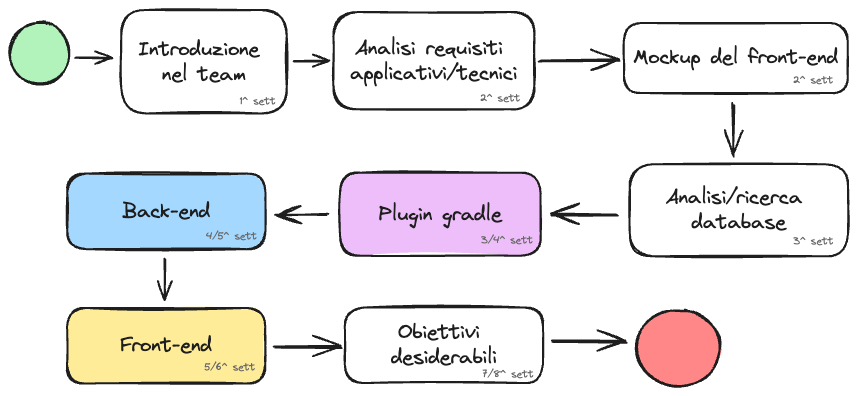
\includegraphics[width=1\columnwidth]{workflow-stage} 
  \caption{Sequenza temporale delle attività svolte durante lo \textit{stage}.}
  \label{fig:workflow-stage}
\end{figure}

L'identificazione degli obiettivi e delle aspettative è un passo fondamentale per la definizione di un progetto di \textit{stage}.
In questo contesto, gli obiettivi rappresentano le funzionalità che il sistema deve implementare, mentre le aspettative
sono le caratteristiche che il sistema deve possedere.\\
Gli obiettivi e le aspettative del progetto di \textit{stage} sono stati definiti in collaborazione con il tutor aziendale, 
tramite il piano di lavoro.
Esso è stato redatto prima dell'inizio dello \textit{stage}, e ha rappresentato un punto di riferimento per la valutazione
delle attività svolte durante il periodo di \textit{stage}.\\
All'interno del piano di lavoro erano presenti obiettivi obbligatori e obiettivi desiderabili.
Gli obiettivi avevano un codice identificativo, e una descrizione.\\ 
Il codice identificativo era composto da una lettera che rappresentava la tipologia di obiettivo, e da un numero progressivo.
Il progressivo ha permesso l'ordinamento, non casuale, degli obiettivi. \\
La pianificazione settimanale scritta nel piano di lavoro è stata una vera e propria guida per lo svolgimento delle attività, ed 
ha permesso di rispettare le scadenze, raggiungendo gli obiettivi prefissati in ordine di priorità, portando quelli desiderabili
a termine solo se il tempo lo permetteva.\\

Nel piano di lavoro gli obiettivi non erano molto dettagliati, questo ci ha permesso di avere una certa flessibilità durante lo svolgimento
delle attività, e di poter cambiare gli obiettivi in corso d'opera, se necessario.\\

\begin{table}[!h]
  \caption{Obiettivi obbligatori}
  \label{tab:obiettivi-obbligatori}
\begin{tabularx}{\textwidth}{lX}
   \textbf{Identificativo}&\textbf{Descrizione}\\ 
    \hline O01&Analisi dell'attuale infrastruttura\\
    \hline O02&Analisi requisiti applicativi e tecnici e \textit{mockup} del \textit{front end}\\
    \hline O03&Identificazione del db a grafo più adeguato al progetto\\
    \hline O04&Implementazione della struttura di \textit{database}\\
    \hline O05&Implementazione di un \textit{plugin gradle} per la raccolta delle informazioni\\
    \hline O06&Invocazione da \textit{jenkins}\\
    \hline O07&Implementazione dei servizi \textit{backend} per l'interrogazione del sistema\\
    \hline O08&Implementazione del \textit{front end} per rendere possibile l'interrogazione\\
    \hline 
\end{tabularx}
\end{table}

  \begin{table}[!h]
    \caption{Obiettivi desiderabili}
    \label{tab:obiettivi-desiderabili}
    \begin{tabularx}{\textwidth}{lX}
    \textbf{Identificativo}&\textbf{Descrizione}\\ 
    \hline D01&Possibilità di visualizzare i risultati in forma grafica (grafo) e non solo tabellari\\
    \hline D02&Integrazione con \textit{repository} remoti al fine di verificare nuove versioni delle dipendenze\\
    \hline D03&Integrazione con \textit{repository} remoti al fine di identificare vulnerabilità sulle dipendenze utilizzate\\
    \hline D04&Login con \textit{LDAP} aziendale\\  
    \hline
  \end{tabularx}
  \end{table}



  \section{Vincoli}
  \subsection*{ Vincoli tecnologici}

  Il piano di lavoro tramite gli obiettivi, intrinsecamente, ha definito i vincoli tecnologici del progetto.\\
  Il primo vincolo è stato quello di utilizzare un \textit{database} a grafo per il salvataggio dei dati raccolti dal \textit{plugin},
  questo perchè permette di rappresentare le dipendenze in maniera naturale, e di eseguire \textit{query} molto complesse in tempi molto brevi.\\
  Con i membri del team abbiamo deciso di utilizzare \textit{Neo4j} come \textit{database} a grafo, perchè è il più utilizzato, ha una comunità molto attiva
ed è molto ben documentato.

Il secondo vincolo tecnologico è stato quello di utilizzare \textit{Gradle} per il \textit{plugin} che raccoglie le informazioni sulle dipendenze,
questo perchè quasi tutti i progetti di {\azienda} lo utilizzano come sistema di build.\\

\subsubsection*{Gralde}
  \textit{Gradle} è uno strumento di automazione della \textit{build} \textit{open source} che si è guadagnato una notevole popolarità nel mondo 
dello sviluppo \textit{software}, grazie alla sua flessibilità e potenza. Utilizzato principalmente per progetti \textit{Java}, 
è anche ampiamente adottato per applicazioni scritte in altri linguaggi di programmazione come \textit{Kotlin}, \textit{C++}, e \textit{Python}. 
La sua caratteristica principale è la capacità di supportare configurazioni di \textit{build} altamente personalizzabili, 
rendendolo adatto sia per piccoli progetti sia per grandi imprese con esigenze complesse.

\textit{Gradle} si distingue per l'uso di un \gls{DSLg} basato sui linguaggi di programmazione \textit{Groovy} o \textit{Kotlin},
 che fornisce un modo intuitivo e dichiarativo di definire le \textit{build}. Questo approccio, combinato con la sua potente capacità di 
 gestione delle dipendenze e il suo modello di esecuzione incrementale, consente agli sviluppatori di costruire \textit{software} in modo più 
 efficiente e affidabile. Inoltre, \textit{Gradle} è noto per la sua velocità, superando spesso altri strumenti di \textit{build} come \textit{Maven} 
 e \textit{Ant}, specialmente in progetti di grandi dimensioni.

 \begin{figure}[!h] 
  \centering 
  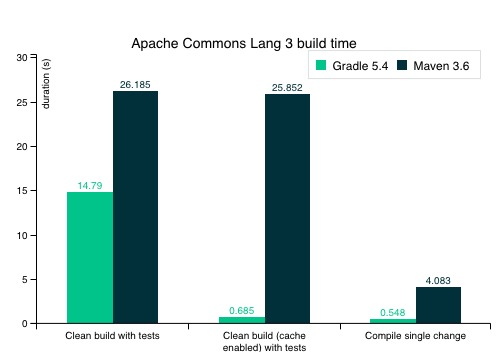
\includegraphics[width=1\columnwidth]{gradle-vs-maven.jpeg} 
  \caption{Comparazione tra \textit{Gradle} e \textit{Maven}. Fonte: https://gradle.org/maven-vs-gradle}
  \label{fig:gredle-vs-maven}
\end{figure}

Un altro aspetto fondamentale di \textit{Gradle} è la sua estensibilità. Gli sviluppatori possono estendere le funzionalità di \textit{Gradle} 
scrivendo script personalizzati o integrando \textit{plugin} esistenti. Questa flessibilità lo rende uno strumento ideale per adattarsi a 
flussi di lavoro specifici e requisiti di \textit{build} unici. Gradle è anche il sistema di \textit{build} ufficiale per \textit{Android}, ulteriormente 
consolidando la sua posizione come uno strumento chiave nello sviluppo di applicazioni moderne.

\subsubsection*{\textit{Angular}}
Un altro vincolo tecnologico è stato quello di utilizzare \textit{Angular} per lo sviluppo del \textit{frontend}, 
questo perchè, come scritto precedentemente, è il \textit{framework} più utilizzato in azienda per lo sviluppo delle \textit{web-app}.\\

\textit{Angular} è un \textit{framework} \textit{front-end} \textit{open source} sviluppato e mantenuto da \textit{Google}. 
È ampiamente riconosciuto per la sua capacità di creare applicazioni \textit{web} dinamiche e reattive. 
\textit{Angular} utilizza \textit{TypeScript}, una \textit{super-set} di \textit{JavaScript}, che fornisce funzionalità di tipizzazione statica e 
orientamento agli oggetti, migliorando la manutenibilità e la qualità del codice.

Una delle caratteristiche distintive di \textit{Angular} è il suo approccio basato su componenti, che aiuta gli sviluppatori a 
costruire applicazioni \textit{web} complesse in modo più modulare e mantenibile. Ogni componente in \textit{Angular} è una combinazione di \textit{HTML}, 
\textit{CSS}, e \textit{TypeScript}, che gestisce una parte specifica dell'interfaccia utente. Questo approccio promuove la riusabilità 
del codice e una migliore separazione delle preoccupazioni.

\textit{Angular} è anche noto per il suo potente sistema di \textit{dependency injection}, che semplifica lo sviluppo e il \textit{testing} fornendo un 
modo per iniettare dipendenze in classi in modo pulito e flessibile. Inoltre, \textit{Angular} offre un'ampia gamma di funzionalità integrate come il 
\textit{routing}, la gestione delle \textit{form}, e l'accesso HTTP, che accelerano lo sviluppo di applicazioni textit{web}.

\begin{figure}[h] 
  \centering 
  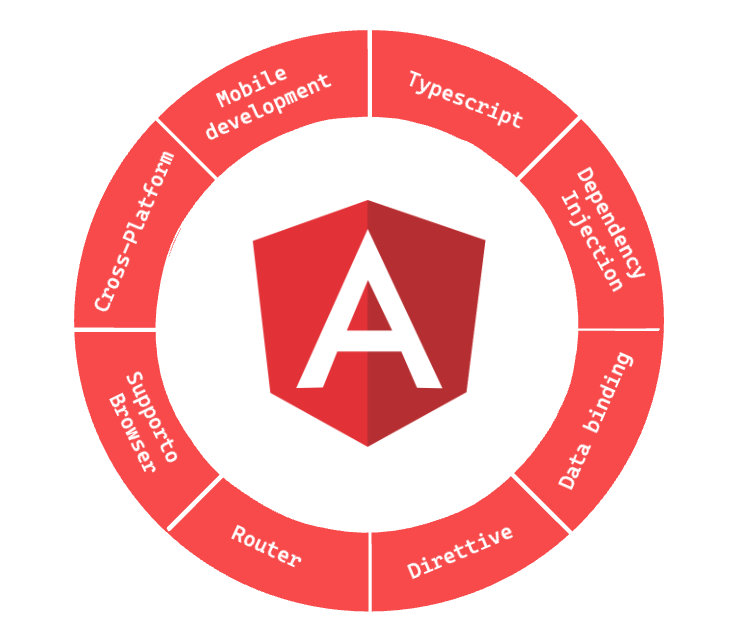
\includegraphics[width=0.5\columnwidth]{feature-angular.png} 
  \caption{Caratteristiche di \textit{Angular}.}
  \label{fig:workflow-stage}
\end{figure}

Con il suo ecosistema ricco e una forte comunità di sviluppatori, \textit{Angular} è diventato uno dei \textit{framework} \textit{front-end} più popolari e 
affidabili per lo sviluppo di applicazioni \textit{web} moderne, sia per progetti di piccole dimensioni sia per applicazioni aziendali di grande scala.

\subsubsection*{I database a grafo e \textit{Neo4j}}

I \textit{database} a grafo sono una categoria di \textit{database} NoSQL progettati per gestire e rappresentare dati complessi e le loro relazioni 
in modo più efficiente rispetto ai tradizionali \textit{database} relazionali. Questi \textit{database} utilizzano strutture di grafo per la memorizzazione 
semantica, con nodi, bordi e proprietà per rappresentare e memorizzare dati. La flessibilità dei \textit{database} a grafo li rende particolarmente 
adatti per applicazioni che richiedono l'analisi di relazioni complesse e interconnesse, come i \textit{social network}, i sistemi di raccomandazione, 
e la gestione delle reti.

\textit{Neo4j} è uno dei più popolari \textit{database} a grafo, noto per la sua alta \textit{performance} e flessibilità. È un \textit{database} \textit{open source}, 
ma offre anche una versione \textit{enterprise} con funzionalità aggiuntive. \textit{Neo4j} utilizza il linguaggio di \textit{query} \textit{Cypher}, che è specificamente 
progettato per lavorare con grafi. \textit{Cypher} consente agli sviluppatori di esprimere facilmente \textit{query} complesse sulle relazioni tra i dati, 
rendendo \textit{Neo4j} particolarmente potente per analisi di dati relazionali complessi.

\begin{figure}[h] 
  \centering 
  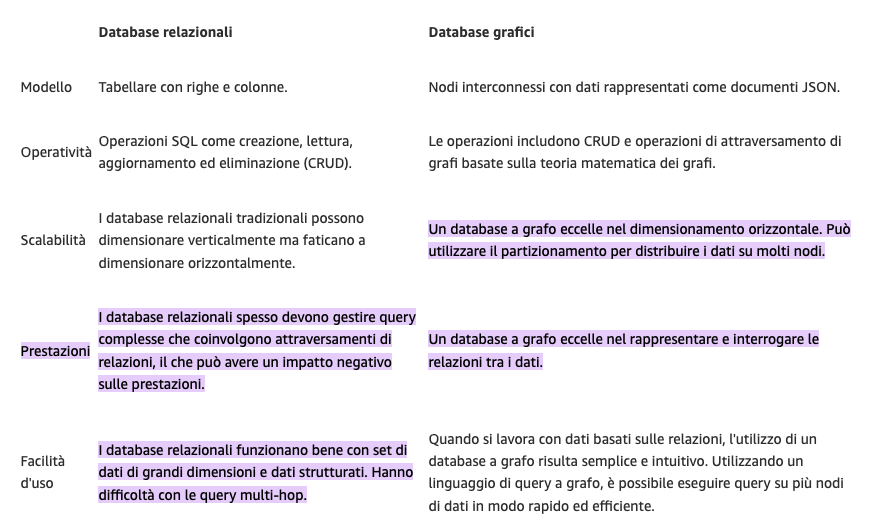
\includegraphics[width=1\columnwidth]{graphdb-vs-sql.png} 
  \caption{Differenze tra \textit{database} a grafo e \textit{database} relazionali. \\Fonte: https://aws.amazon.com/it/compare/the-difference-between-graph-and-relational-database.}
  \label{fig:graphdb-vs-sql}
\end{figure}

\subsection*{ Vincoli di dominio}
Il proddotto finale dovrà essere utilizzato, non solo dagli sviluppatori, ma anche dai \textit{project manager}, i \textit{team leader}, e i \textit{product owner} ed
i consulenti; Per questo è stato richiesto, come obiettivo desiderabile, di implementare l'autenticazione tramite \textit{LDAP} aziendale, 
per permettere l'accesso a tutti i dipendenti di {\azienda}.\\
L'\textit{LDAP} è un protocollo di rete che permette la gestione centralizzata delle autenticazioni e delle autorizzazioni.
Questo è fondamentale per garantire la sicurezza dei dati, e per permettere l'accesso solo a chi ne ha i permessi, senza dover
implementare un sistema di autenticazione ad hoc.\\



\section{La scelta dello stage}
La scelta dello stage non è stata molto semplice. La scelta principale da fare era, se scegliere un progetto interno all'azienda, o 
se momentaneamente abbandonare l'azienda per fare l'esperienza di stage in un'altra azienda.\\ 
Lo stage per me rappresenta un'opportunità per imparare nuove tecnologie, e per mettermi alla prova in un ambiente lavorativo diverso 
e questa poteva essere l'occasione giusta. Dopo aver valutato i pro e i contro, ho deciso di rimanere in azienda, perchè siamo riusciti
a trovare un progetto molto interessante e stimolante, che mi ha permesso di imparare nuove tecnologie, e di mettermi alla prova.\\

Questo progetto avrebbe permesso di affrontare problemi riguardanti lo sviluppo \textit{software}, problemi di gestione e organizzazione del lavoro ma 
anche i problemi riguardanti i sistemi di \textit{build} e di \textit{continuous integration}, un argomento che mi ha sempre affascinato ma che non ho mai
avuto modo di approfondire.\\

\section{Pianificazione e interazioni con il tutor}
All'inizio dello \textit{stage} ho avuto un incontro con il tutor aziendale, per discutere del piano di lavoro, e per definire la modalità
di svoldimento e di interazione durante lo \textit{stage}.\\
Abbiamo deciso di fare un incontro settimanale, per discutere delle attività svolte durante la settimana, e per pianificare le attività
della settimana successiva.\\
Quando avevo dei dubbi o dei problemi, potevo contattarelo tramite \textit{Google Chat} o tramite \textit{email}.\\
Ogni mattina alle 9:00 avevamo un incontro con il \textit{team} di sviluppo, per discutere delle attività svolte il giorno precedente, e per
pianificare le attività della giornata, come previsto dalla metodologia \textit{Agile}.\\
A questo incontro non partecipava il tutor aziendale. 
Capitava spesso comunque di avere degli incontri al di fuori di quelli pianificati, per discutere di problemi, principalmente analitici, 
e per prendere decisioni riguardanti l'implementazione.\\

\begin{figure}[h] 
  \centering 
  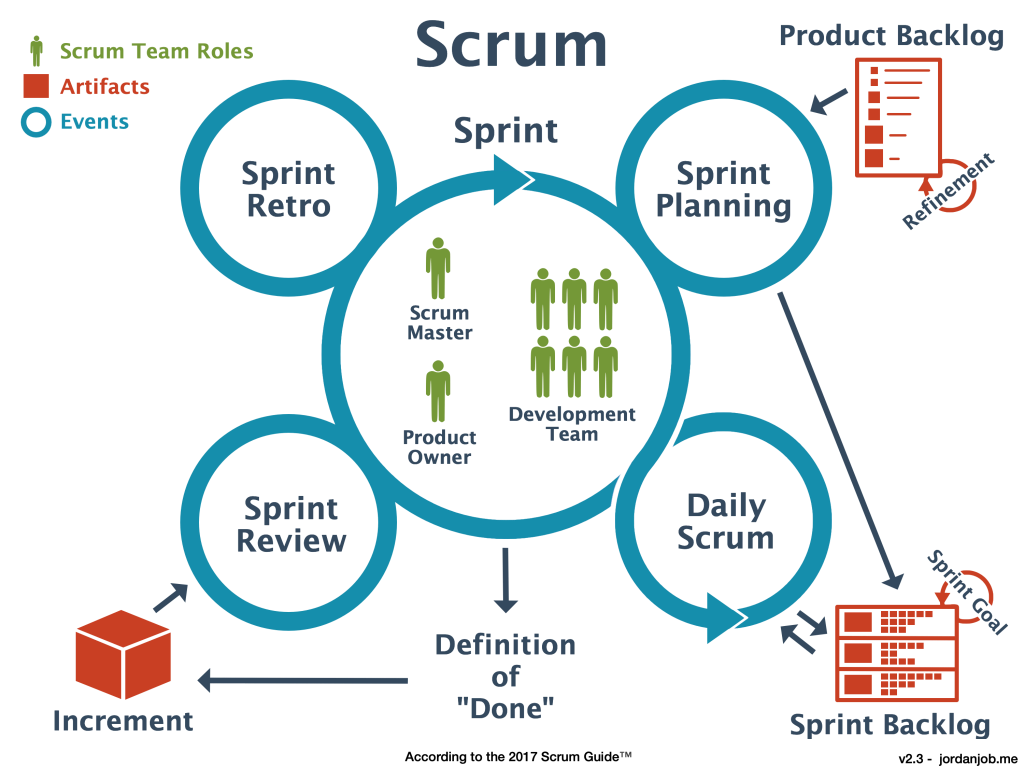
\includegraphics[width=.8\columnwidth]{scrum_agile.png} 
  \caption{Metodologia \textit{Agile}. Fonte: https://jordanjob.me/blog/scrum-diagram. }
  \label{fig:scrum_agile}
\end{figure}